\documentclass[tikz]{standalone}
\usepackage{../customcommand}
\usetikzlibrary{arrows,positioning}
\tikzset{
    >=stealth', % standard arrow tip
    box/.style={
           rectangle,
           rounded corners,
           draw=black,
           very thick,
           text width=4.5em,
           text centered,
           minimum height=2.5em},
    arrowlabel/.style={
        text width=4em,
        outer sep=0.5em,
        label={\scriptsize}},
    arrow/.style={
           ->,
           thick,
           bend left=90,
           distance=3.5em,
           shorten <=1pt,
           shorten >=2pt,}
}


\begin{document}
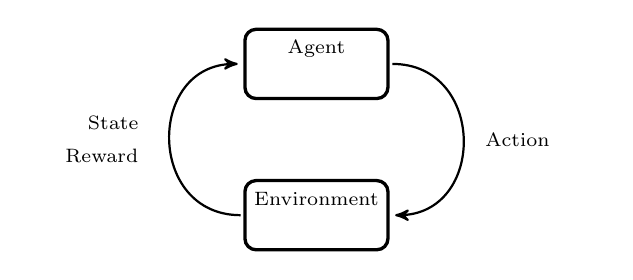
\begin{tikzpicture}[node distance=1cm, auto,]
    % Nodes
    \node[box]                 (agent)       {\scriptsize Agent \\ $\agent$};
    \node[box, below=of agent] (environment) {\scriptsize Environment \\ $\environment$};
    % Edges
    \path
        (agent.east)       edge[arrow] node[arrowlabel, align=left ]{\scriptsize Action $\action$}                   (environment.east)
        (environment.west) edge[arrow] node[arrowlabel, align=right]{\scriptsize State $\state$ \\ Reward $\reward$} (agent.west);
\end{tikzpicture}
\end{document}
